\section{Mesh generation on spherical manifolds}
\label{sect:spherical_manifolds}
\par

In this example, we generate a mesh of a section of the ocean on the surface of a sphere (the Earth). Within just a few steps, we will be able to produce a mesh
similar to figure~\ref{fig:sphericalpatch}.

\begin{figure}[htbp]
 \centering
  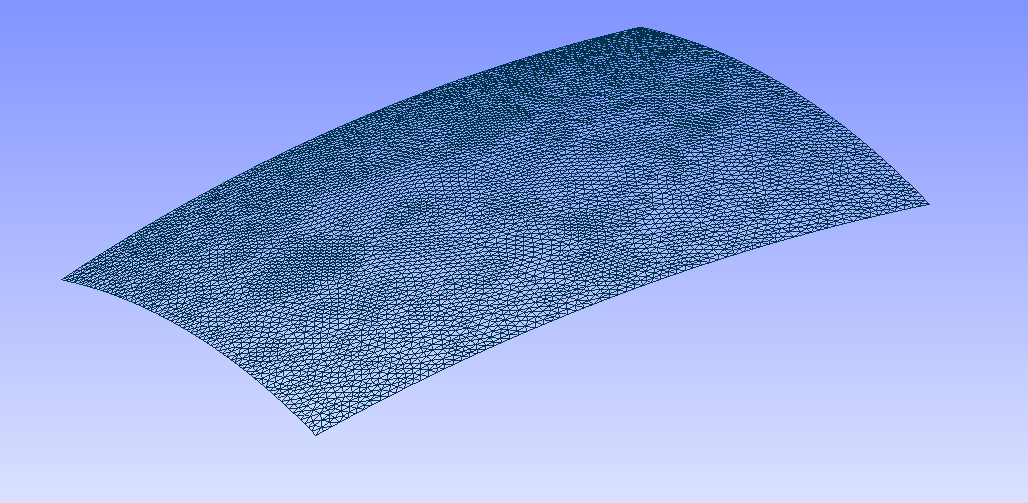
\includegraphics[width=1.0\textwidth]{../figures/sphericalpatch}
  \caption{A 2--D manifold in 3--D space.}
  \label{fig:sphericalpatch}
\end{figure}

We will make primary use of the Gmsh scripting language and resort to the graphical user interface only to ensure that we are progressing correctly. We will be saving the script with the .geo extension, which Gmsh recognises as its own. To generate a file manifold.geo, we may issue:
\begin{lstlisting}
gedit manifold.geo
\end{lstlisting}
which opens the gedit text editor and generates the manifold.geo file.

In this chapter you will learn how to:
\begin{enumerate}
\item Define points on the sphere (section~\ref{sect:definepointsmanifold}).
\item Connect the points with lines (section~\ref{sect:definelinesmanifold}).
\item Define physical surfaces and generate meshes on the sphere (section~\ref{sect:meshgenerationmanifold}).
\end{enumerate}

First, however, we will be introducing the process of stereographic projection (section~\ref{sect:stereoprojection}). This is important because we need to define points on the projected plane before Gmsh automatically maps them back to the sphere.

\subsection{Background: Stereographic projection}
\label{sect:stereoprojection}
A stereographic projection, $\sigma$, maps all points (apart from one, the \emph{North Pole}) of an $n$--dimensional unit sphere, $S^n \in  R^{n+1}$, to an $n$--dimensional plane:
%%
\begin{align}
\sigma : S^n \rightarrow R^n
\end{align}
%%
Figure~\ref{fig:2dstereoprojection} illustrates a two-dimensional sphere being projected onto a line.

\begin{figure}[htbp]
 \centering
  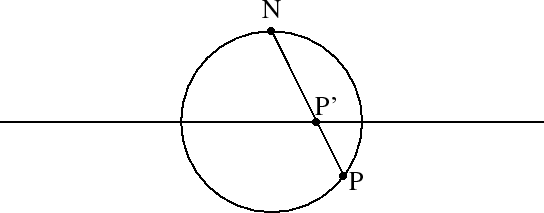
\includegraphics[width=0.9\textwidth]{../figures/2dstereoprojection}
  \caption{2--D stereographic projection. Point N indicates the North Pole. Point P` is the projection of Point P.}
  \label{fig:2dstereoprojection}
\end{figure}

%Don't forget to cite the Wolfram Alpha website.

\subsection{Defining Points}
\label{sect:definepointsmanifold}
Gmsh has the capability of plotting points on the sphere. To the user`s convenience, only the projections of these points need to be defined. Prior to these points, however, two special points are required:
\begin{enumerate}
  \item The center of the sphere.
  \item The \emph{North Pole}.
\end{enumerate}

To start our example, open a plain file and begin by defining the special points described:
\begin{lstlisting}
Point(1) = {0.0,0.0,0.0};         //The center of the sphere
Point(2) = {0.0,0.0,6.37101e+06}; //The North Pole
\end{lstlisting}
We then need to inform Gmsh that any further points defined, will be on the sphere. So we issue the following statement:
\begin{lstlisting}
PolarSphere(1) = {1,2}; //Sphere with center at Point(1)
                        //and North Pole at Point(2).
\end{lstlisting}

We now proceed by defining the remaining points, with coordinates on the 2--D plane. In this example, we will create a domain that spans from +10 to +30 degrees in longitude and +5 to +25 in latitude.

\begin{lstlisting}
//Point 3: 10 lon 5 lat

//First we convert to radians
//and then to stereographic coordinates.
Point_lon_rad = (10)*(Pi/180);
Point_lat_rad = (5)*(Pi/180);
Point_3_stereographic_x = -Cos(Fabs(Point_lon_rad))*Cos(Fabs(Point_lat_rad))/
    ( 1 + Sin(Fabs(Point_lat_rad)) );
Point_3_stereographic_y = Cos(Fabs(Point_lat_rad))*Sin(Fabs(Point_lon_rad))/
    ( 1 + Sin(Fabs(Point_latx_rad)) );

//Now we define the point
Point(3) = {Point_stereographic_x, Point_stereographic_y,0};
\end{lstlisting}

We must repeat the process for the remaining three points:
\begin{itemize}
\item[-] Point 4: 10 lon 25 lat
\item[-] Point 5: 30 lon 25 lat
\item[-] Point 6: 30 lon 5 lat
\end{itemize}

After we have defined the center, north pole and 4 edges of our domain; it is sensible to open up the file in Gmsh to have a look at our progress. We first save the file and then open it in Gmsh by issuing the following command at the terminal:
\begin{lstlisting}
gmsh manifold.geo
\end{lstlisting}
The center and north pole should be visible, as well as the 4 points on the surface of the sphere, as in figure~\ref{fig:pointsdefinition}.

\begin{figure}[htbp]
 \centering
  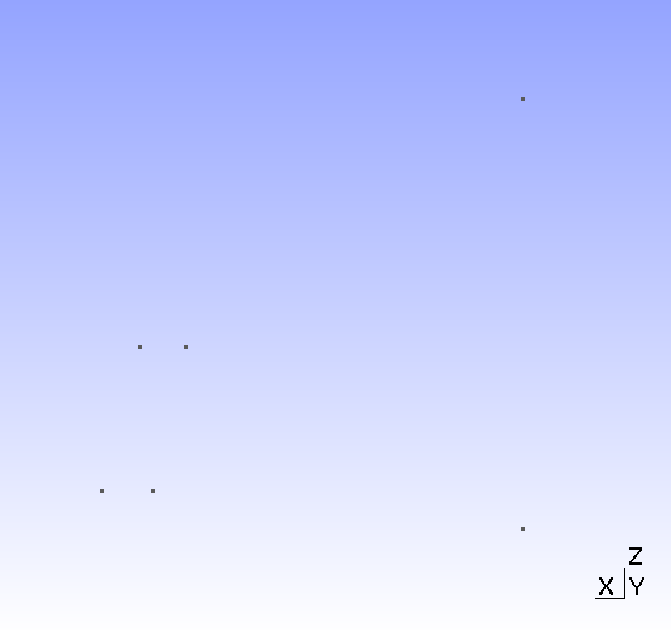
\includegraphics[width=0.9\textwidth]{../figures/pointsdefinition}
  \caption{The center of the sphere (below right), as well as the North pole (top right) and the four edges of the domain are visible in Gmsh. It is clear by looking at the coordinate system that the four points have been mapped from the 2--D plane.}
  \label{fig:pointsdefinition}
\end{figure}

\subsection{Defining zonal and meridional lines}
\label{sect:definelinesmanifold}
In stereographic projection of a 2--D sphere such as the Earth, lines of constant latitude are mapped to straight lines in a plane. Gmsh is therefore able to accurately interpolate meridional lines, given just two points. Lines of constant longitude however, are projected to circles in the plane. The arcs between these points are also approximated by straight lines in Gmsh so a poor result is obtained if the distance between the points is large.

To correct this problem, we break any zonal paths into smaller segments for which the straight line assumption is valid. We will be using the following function:
\begin{lstlisting}
Function DrawParallel
 alpha = parallelSectionStartingY/parallelSectionStartingX;
 parallelRadius = Sqrt(parallelSectionStartingX^2 + parallelSectionStartingY^2);
 deltaAlpha = (parallelSectionEndingY/parallelSectionEndingX - 
    parallelSectionStartingY/parallelSectionStartingX)/pointsOnParallel;
 For t In {1:pointsOnParallel}
  alpha += deltaAlpha;
  newParallelPointX = (parallelSectionStartingX/Fabs(parallelSectionStartingX))
     *parallelRadius/(Sqrt(alpha^2 + 1));
  newParallelPointY = newParallelPointX*alpha;
  newPointOnParallel = newp;
  Point(newPointOnParallel) = {newParallelPointX, newParallelPointY, 0};
 EndFor
 BSpline(newParallelID) = {firstPointOnParallel, newPointOnParallel-
     (pointsOnParallel-1):newPointOnParallel, lastPointOnParallel};
Return
\end{lstlisting}

The function we have just defined requires the following parameters to be set prior to being called:
\begin{itemize}
\item pointsOnParallel : The number of points to be defined between the two we have already defined.
\item parallelSectionStartingX : The first stereographic coordinate of the starting point. If we are drawing the southernmost zonal line, this will be the x-coordinate of the south-westernmost point (Point(3) in our case). The Y coordinate is also required in a respectively named parameter, as well as the X and Y coordinates of the ending point (south-easternmost point, Point(6)).
\item firstPointonParallel : In addition to its coordinates, the function needs to know the point number of the first and last points of the zonal line.
\item newParallelID : Finally, each line we draw needs a unique number.
\end{itemize}

We can now go ahead and plot the zonal lines by appending the following to our manifold.geo file:

\begin{lstlisting}
//Draw south-most parallel of the Domain. Point 3 to Point 6

//Assign parameters to variables and then call function DrawParallel,
pointsOnParallel = 200;
parallelSectionStartingX = Point_3_stereographic_x;
parallelSectionStartingY = Point_3_stereographic_y;
firstPointOnParallel = 3;
parallelSectionEndingX = Point_6_stereographic_x;
parallelSectionEndingY = Point_6_stereographic_y;
lastPointOnParallel = 6;
newParallelID = 1;
Call DrawParallel;
\end{lstlisting}

The meridional lines are much simpler, and can be drawn by simply specifying to Gmsh that we require a B-spline between the two points:

\begin{lstlisting}
//Draw western-most meridional
BSpline(3) = {3, 4};
//Draw eastern-most meridional
BSpline(4) = {5, 6};
\end{lstlisting}

Saving and opening the manifold.geo file in Gmsh should now look like what we see in figure~\ref{fig:linesdefinition}.

\begin{figure}[htbp]
 \centering
  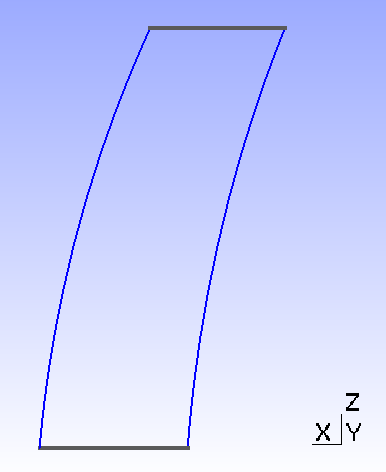
\includegraphics[width=0.7\textwidth]{../figures/linesdefinition}
  \caption{The points of figure~\ref{fig:pointsdefinition} have now been connected by lines. Note that zonal lines have had points defined along their path, as requested in the function we defined.}
  \label{fig:linesdefinition}
\end{figure}


\subsection{Mesh generation}
\label{sect:meshgenerationmanifold}
All that remains to generate the mesh is to specify the Physical surface and a Field to instruct Gmsh of the desired element length.

\begin{lstlisting}
//Define new line from previously generated lines that generates a loop.
Line Loop(6) = {3,2,4,-1};
Plane Surface(7) = {6}; //Surface from Loop
Physical Surface(8) = {7};

Field[50] = MathEval; //Generate Field
Field[50].F = "30000";
Background Field = 50;
\end{lstlisting}

The variable \lstinline{Field[50].F} should equal the desired element edge size. In our example, we set it equal to a constant \lstinline{30000} indicating we want a constant element edge size of $30km$. This value could have been any other mathematical expression to be evaluated by Gmsh.

We can now instruct Gmsh to mesh the defined domain by issuing the following command at the terminal:
\begin{lstlisting}
gmsh -3 manifold.geo
\end{lstlisting}
This will produce a file manifold.msh which can be opened in Gmsh. This will give you a mesh such as that shown in figure~\ref{fig:sphericalpatch}.

The full .geo file used in this example is given:

\lstinputlisting{../figures/spherical_manifold_example.txt}
